Os simuladores de realidade virtual aumentaram a capacidade de testar cenários de RVD/B, reduzindo custos e riscos de testes em órbitas, além de proporcionar maior facilidade pois pode ser realizado em praticamente qualquer computador com o mínimo de poder computacional requerido pelas principais plataformas de simulação.

\subsection{Ambientes virtuais}

A plataforma Gazebo \citep{gazebo2025} é conhecida no meio acadêmico por ser versátil e precisa, além de proporcionar liberdade para construir cenários e situações desejadas para observar o funcionamento e ajustá-las conforme a necessidade.

\subsection{Gazebo}

O Gazebo trata-se de uma plataforma de simulação utilizada no desenvolvimento e teste de sistemas robóticos em ambientes virtuais antes da implementação em hardware real. A sua elevada capacidade de modelagem física permite a criação de cenários (ou mundos, como são conhecidos) complexos, nos quais robôs podem ser testados sob diferentes condições ambientais, o que auxilia a reduzir os riscos e custos relacionados aos experimentos no mundo real. A plataforma suporta a integração com diversos sensores e atuadores, proporcionando uma representação próximo do real no que se diz sobre as interações entre os robôs e o mundo. Além disso, sua compatibilidade com o Robot Operating System (ROS) facilita o desenvolvimento e a implementação de algoritmos de controle e navegação.

Tratando-se de aplicações espaciais, o Gazebo pode ser utilizado para simular operações de robôs em ambientes de microgravidade ou superfícies planetárias. Isso possibilita o teste de algoritmos de locomoção para rovers em terrenos irregulares, bem como a avaliação de estratégias para manipulação de objetos em baixa gravidade. Realizar a simulação dessas condições é essencial para o desenvolvimento de missões espaciais, permitindo ajustes finos nos sistemas de controle antes do envio dos equipamentos ao espaço. A plataforma também possibilita a criação de cenários colaborativos, onde múltiplos agentes (robôs autônomos e operadores humanos) podem interagir em um ambiente simulado, explorando todas as possibilidades para as missões de exploração e manutenção orbital.

Ademais, uso da plataforma Gazebo se estende à robótica humanoide, permitindo a modelagem de robôs antropomórficos\footnote{Seres ou objetos que têm características humanas ou que se assemelham a um ser humano} para operações que exigem destreza e/ou controle preciso. A implementação de modelos detalhados, como o AR601M, demonstra o potencial da plataforma para simular as habilidades motoras humanas em tarefas colaborativas. Essa abordagem é relevante para a realização de atividades que demandam precisão e repetibilidade em estações espaciais, onde robôs podem auxiliar astronautas nesse tipo de tarefa, resultando em redução na carga de trabalho deles. A possibilidade de testar algoritmos de aprendizado de máquina no ambiente simulado permite a adaptação dos robôs a novas situações sem a necessidade de intervenções diretas.

\begin{figure}[H]
    \centering
    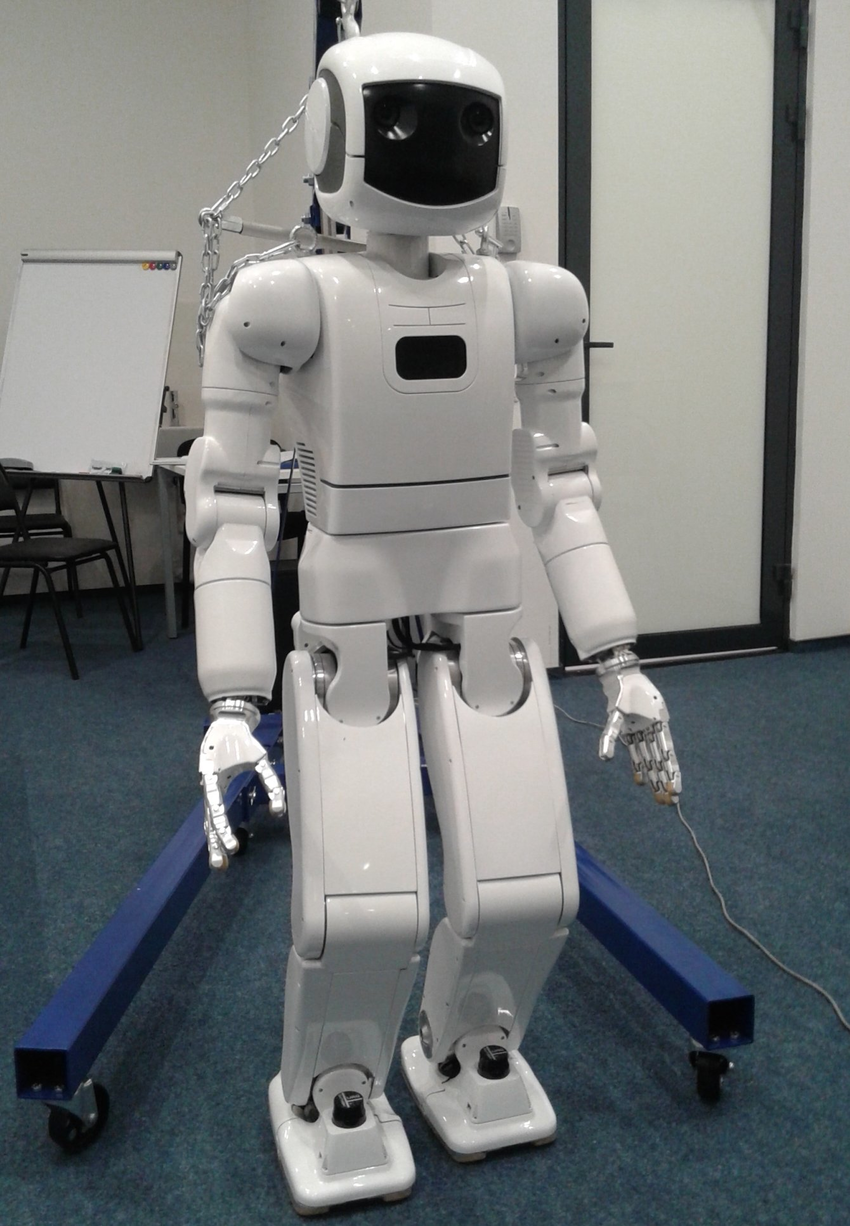
\includegraphics[width=0.75\linewidth]{Imagens/ARM601M.png}
    \caption{Robô antropomórfico AR601M. Fonte: \url{https://www.researchgate.net/figure/Android-Technics-AR-601M-robot_fig3_301721671}}
    \label{fig:AR601M}
\end{figure}

Por fim, a versatilidade, por possuir elevada precisão e por ser de código aberto, o Gazebo acaba se tornando ferramenta valiosa para a pesquisa e desenvolvimento de robôs destinados a ambientes extremos, como o espaço. Utilizando-o na fase de testes e validação ajuda a reduzir a necessidade de experimentação em hardware real, elevando a velocidade de evolução do projeto e de economizar em recursos e espaço físicos para realização dos ensaios e até de acomodação dos materiais, além de possuir documentação para treinamento do pessoal envolvido.

Além disso, outra forma de realizar experimentos de forma econômica, quando comparado com grandes satélites ou até utilizar a ISS para testes diversos é a utilização de CubeSats, que são plataformas modulares, podendo atender de uma unidade (CubeSat 1U) até quantas unidades forem necessárias.
